% \section{Modelo usando el dataset VarQ}

Comenzamos nuestro trabajo analizando el dataset construido en la tesis de Santiago Moreno. Este dataset fue construido inicialmente con las variantes originales del sitio de VarQ \cite{varq}, que consistieron en aproximadamente 400 mutaciones correspondientes a 13 proteínas con 10 variables. Posteriormente en el mismo trabajo se aumentó la cantidad para llegar a las aproximadamente 18 mil variantes del dataset VarQ usando otras fuentes como Clinvar \cite{clinvar} y Humsavar \cite{humsavar}. Llamaremos a este dataset VarQ Completo. 

\section{Variables del dataset VarQ Completo}

A continuación damos una descripción detallada de las variables originales encontradas en el dataset. Presentamos un extracto del trabajo de Santiago Moreno en donde se describen dichas variables: 

\begin{itemize}
    \item Variación de Energía (ENE): En VarQ, las mutaciones son modeladas con el software FoldX \cite{Schymkowitz2005}, que construye un modelo a partir de una estructura dada y luego muta residuos específicos. Luego el software predice el impacto energético de la mutación en la estabilidad de la proteína o, en caso de tratarse de un complejo, en la estabilidad del mismo.
    \item SASA: Es el valor correspondiente a la superficie accesible por parte del solvente, de la cadena lateral del aminoácido. Este valor permite determinar si la cadena lateral se encuentra en la superficie o en el núcleo de la estructura.
    \item Porcentaje de SASA: El porcentaje que representa el SASA sobre el total. Es decir el porcentaje que representa el SASA en función de la estructura de la proteína.
    \item B-Factor (BF): o factor de temperatura, que corresponde a un aminoácido dentro de la proteína. Una mayor temperatura, indica que el aminoácido pertenece a una zona potencialmente de mayor movilidad.
    \item Switchability (SWI): Evalúa cuán propenso a generar un cambio de hélice alfa a hoja beta es un conjunto de aminoácidos \cite{PMID:25082719}.
    \item Aggregability (AGG): El software Tango \cite{Fernandez-Escamilla2004} evalúa cuán
    propenso es un aminoácido a generar agregación en una proteína desde un punto de vista estructural. La agregación es el proceso por el cual proteínas mal formadas
    adoptan una conformación que causa su polimerización en fibrillas agregadas y organizadas. Muchas enfermedades neurodegenerativas, como por ejemplo la Amiloidosis, están asociadas con la agregación proteica.
    \item Conservación (CONS): Se calcula en bits, siempre y cuando la mutación pueda ser mapeada a una posición en una familia PFam asignada \cite{Finn2014}. Cuando una posición tiene un alto valor en bits y la misma posición coincide con el aminoácido conservado en la secuencia de la proteína interpretamos que dicha posición está altamente conservada. La misma puede estar altamente conservada porque es importante estructuralmente o porque es importante para la actividad enzimática \cite{Radusky2017}. Los residuos con alta conservación tendrán un impacto mayor sobre la función pues afectan aminoácidos de la familia.
    \item Sitio Activo (AS): Las posiciones de sitio activo son aquellas que se encuentran marcadas como unidas a ligandos en los archivos PDB o que pertenecen al mismo \textit{pocket} que se encuentren conteniendo estos residuos nombrados o aquellos que pertenezcan al Catalytic Site Atlas \cite{Porter2004}.
    \item Interfaz 3DID: Determina si la posición sirve para una interfaz proteína-proteína según la base de datos de 3DID \cite{Stein2005}.
    \item Interfaz PDB: Determina si la posición sirve para una interfaz proteína-proteína según la base de datos de PDB \cite{Berman2003}.
\end{itemize}


\section{Limpieza del dataset VarQ Completo}

Para trabajar con este dataset decidimos verificar la etiqueta de cada una de las variantes, de manera de confirmar que su status siguiera vigente. Para esto recurrimos a las fuentes Clinvar y Humsavar. Realizamos un primer filtrado de estas tablas quedándonos con aquellas variables con un status confirmado: en el caso de Humsavar, aquellas que figuran con la expresión \textit{Polymorphism} y \textit{Disease}, mientras que en Clinvar nos quedamos con aquellas que figuraban como \textit{Benign} y \textit{Pathogenic}, eliminando aquellas con caracterización difusa, por ejemplo, \textit{Risk Factor} (factor de riesgo). 

\begin{figure}[H]
    \centering
    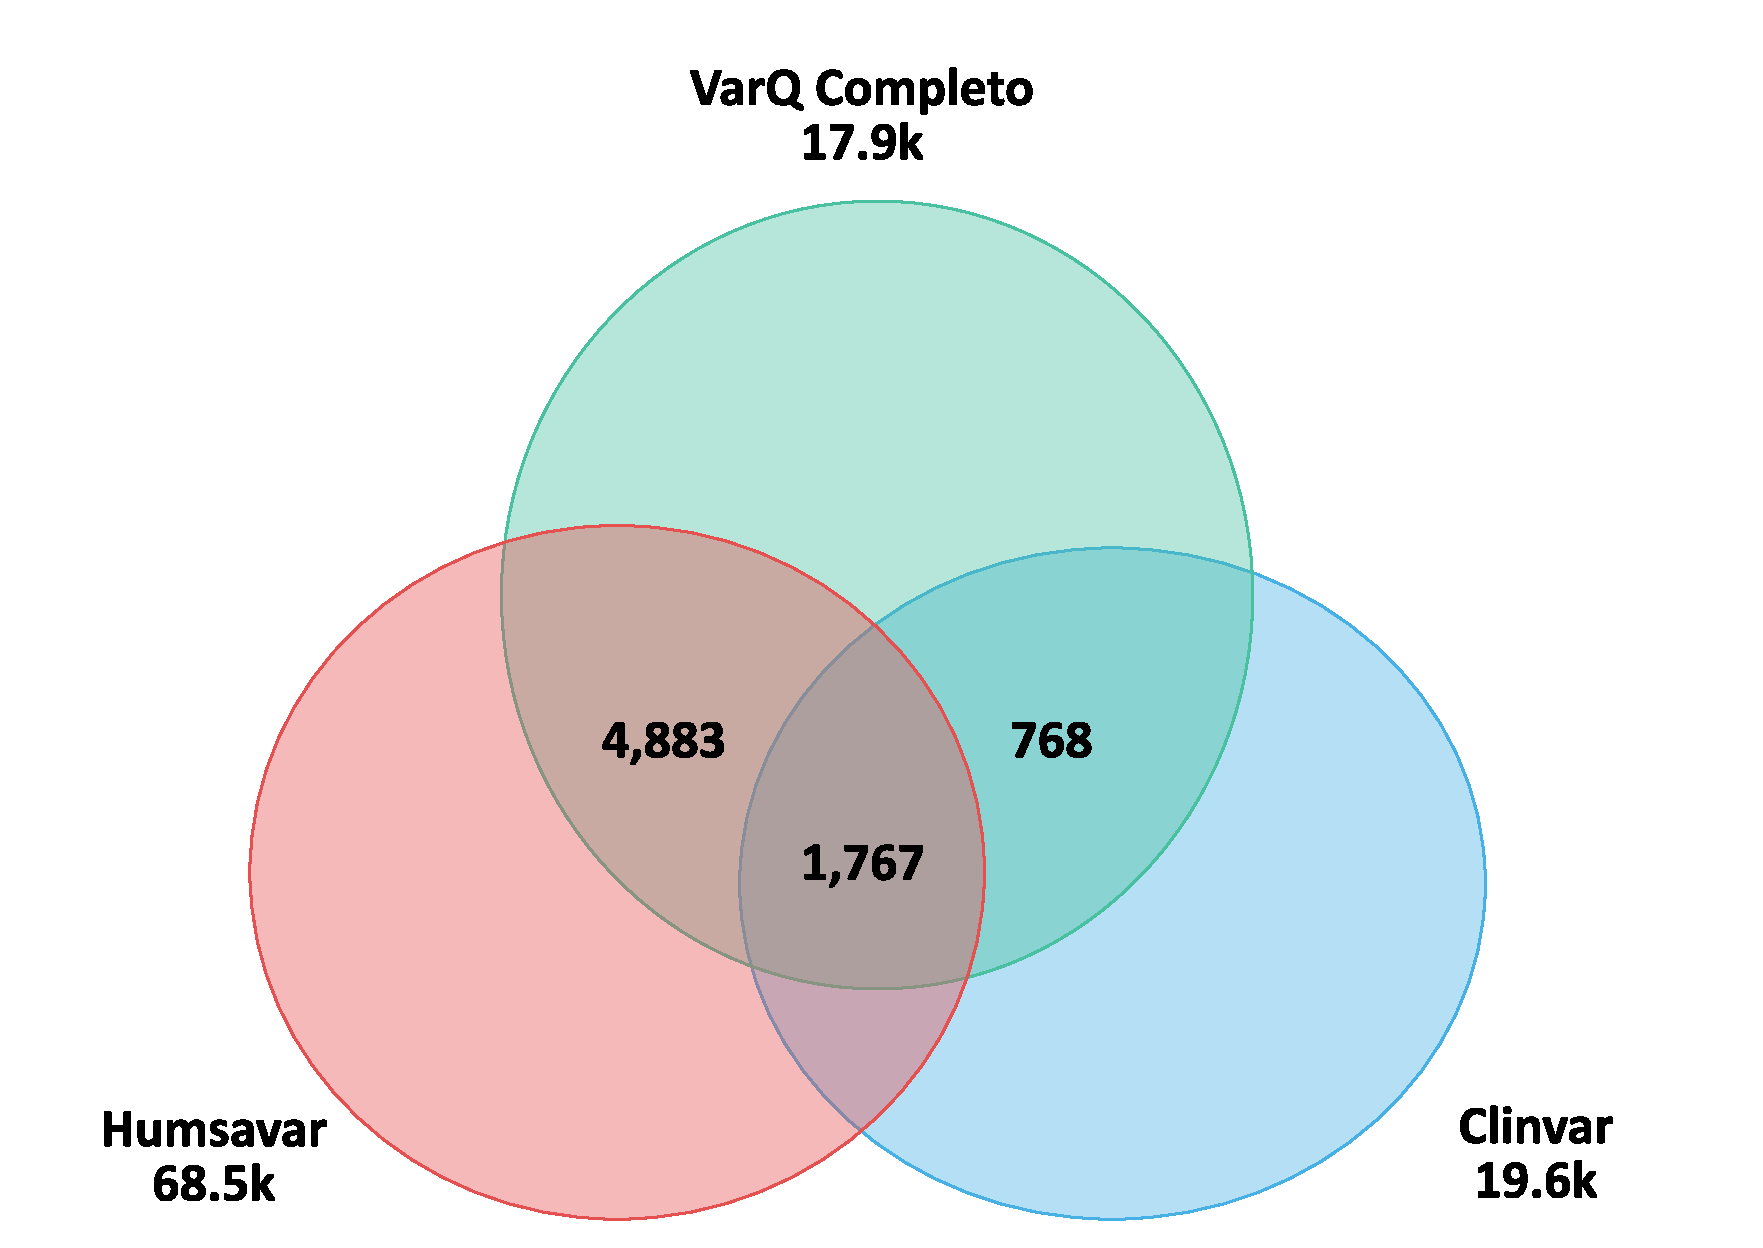
\includegraphics[scale=0.4]{documents/latex/figures/3/varq/interseccion_varq.pdf}
    \caption{Valores en la intersección del dataset VarQ Completo con las tablas Clinvar y Humsavar.}
    \label{fig:interseccion_varq}
\end{figure}

Así, cruzamos los datos con las tablas filtradas Humsavar y Clinvar, y encontramos un subconjunto importante de variantes que no aparecían en ninguna de las dos fuentes. Estas variantes estaban rotuladas en su gran mayoría (94\%) como benignas, por lo que creemos que se consideraron como variantes benignas a todas aquellas a las que no se encontró un reporte. Decidimos remover estas variantes del dataset por considerar que si alguna de ellas estuviera rotulada incorrectamente introduciría ruido. Como puede observarse en la figura \ref{fig:interseccion_varq}, de las 17,869 variantes del dataset VarQ Completo, logramos encontrar 2,535 en la tabla de Clinvar, de los cuales sólo 2,397 tenían un estado confirmado como patogénicas, y 138 como benignas. Cruzando el dataset con la tabla Humsavar encontramos una intersección de 6,650 variantes de los cuales 4,667 corresponden a patogénicas y 1,983 son benignas. Decidimos mantener la clasificación de Humsavar en la intersección de los tres conjuntos por considerarla de mayor confiabilidad dado que es un reporte único curado por expertos, a diferencia de Clinvar que es una recopilación de variantes de diversa significación clínica, y a menudo presenta conflictos de anotación por discrepancias entre evidencias reportadas. Esto nos dejó con un dataset de 7,418 variantes de las cuales 5,377 son patogénicas y 2,041 son benignas. Denominamos a este dataset VarQ Curado. 


\section{Descripción estadística del dataset VarQ Curado}

A partir de VarQ Curado estudiaremos sus variables usando estadísticas descriptivas con el objetivo de evaluar la calidad del dataset. La idea es poder tener una noción de la dispersión de nuestros datos, sumado a la cobertura que tenemos de ellos sobre las variantes.

En la figura \ref{fig:proporcion_nulos_varq} podemos observar cómo la variable de sitio activo (ACTIVE\_SITE) no posee datos para casi ninguna variante (aproximadamente el 95\%), mientras que la variable de conservación (CONS) no posee datos para el 63\% de las variantes. En base a estas observaciones decidimos remover la variable de sitio activo del dataset por considerarla muy poco relevante en términos de cobertura.

\begin{figure}[H]
    \centering
    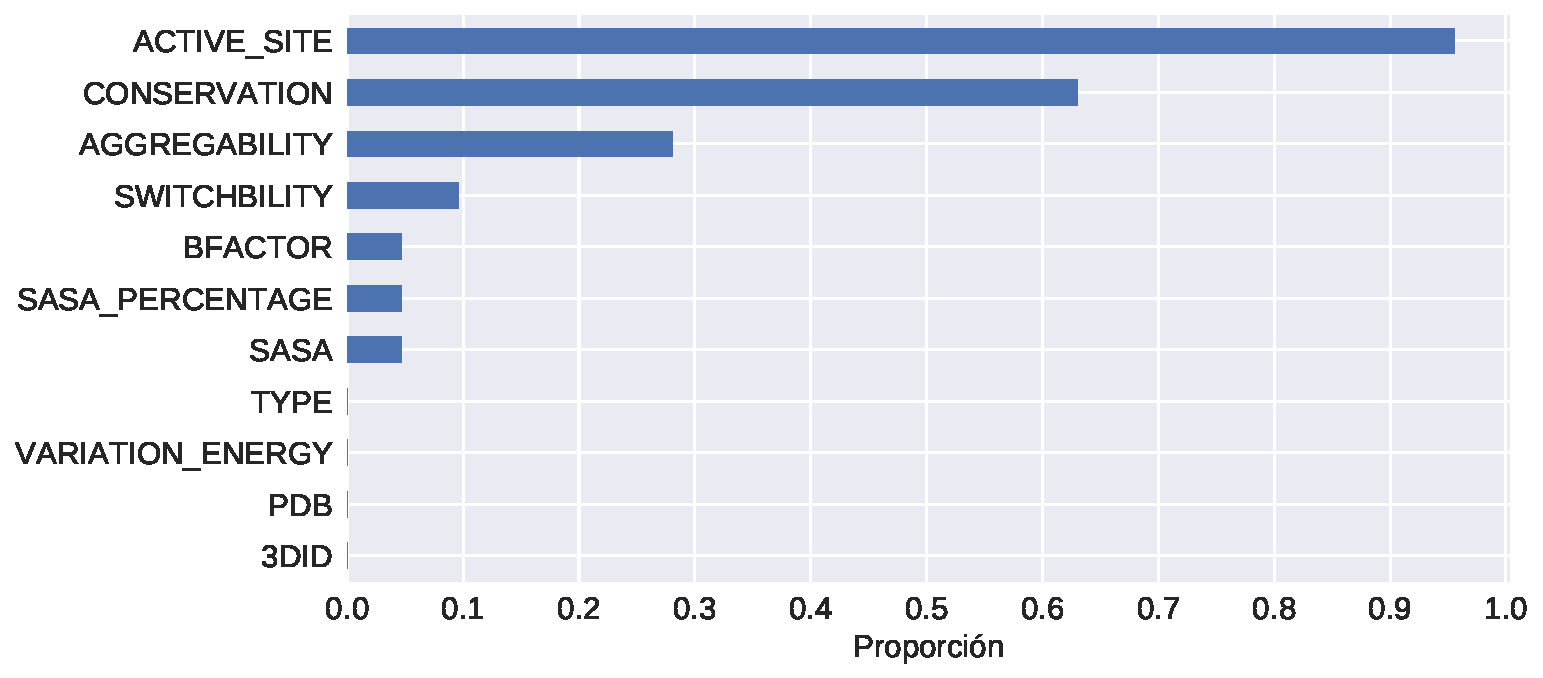
\includegraphics[scale=0.6]{documents/latex/figures/3/varq/proporcion_nulos.pdf}
    \caption{Proporción de variantes con valor nulo por variable del dataset VarQ Curado.}
    \label{fig:proporcion_nulos_varq}
\end{figure}

Otro factor importante a considerar es cuántas variables nulas tienen cada una de las variantes del dataset. En la figura \ref{fig:nulos_varq} podemos observar que existe aproximadamente un 5 \% de variantes que poseen 7 variables nulas de las 10 que contienen el dataset, es decir, prácticamente no tienen ningún tipo de información, y sólo el 2\% de las variantes posee el total de las variables cubiertas. Por el otro lado, casi el 90\% de las variantes tiene a lo sumo 3 variables nulas. Decidimos no remover ninguna fila bajo este criterio.

\begin{figure}[H]
    \centering
    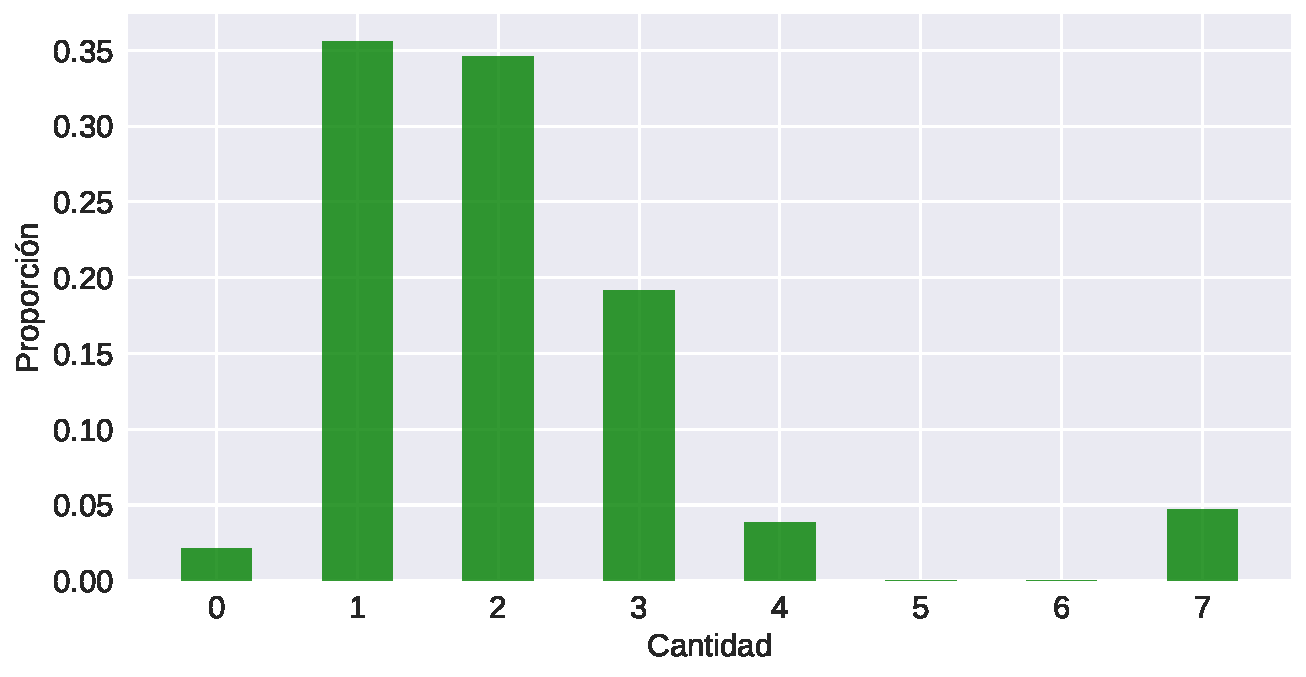
\includegraphics[scale=0.6]{documents/latex/figures/3/varq/nulos_varq.pdf}
    \caption{Histograma de cantidad de variables nulas por fila del dataset VarQ Curado.}
    \label{fig:nulos_varq}
\end{figure}

% \subsection{Correlación entre las variables de VarQ Curado}

También queremos conocer qué tan correlacionadas se encuentras las variables. En la figura \ref{fig:varq_corrplot} vemos la correlación de Spearman que sirve para detectar relaciones monotónicas entre las variables, y así nos permite descartar variables muy similares que no aportan nueva información y ralentizan el entrenamiento del modelo. De esta forma encontramos que la variable SASA y SASA\_PERCENTAGE tienen una correlación de 0.98. Mantuvimos las dos variables dado que la relativa baja cantidad de variables de este dataset no nos fuerza a removerlas, y si bien la correlación es muy alta, no descartamos a priori poder extraer información util usando ambas.

\begin{figure}[H]
    \centering
    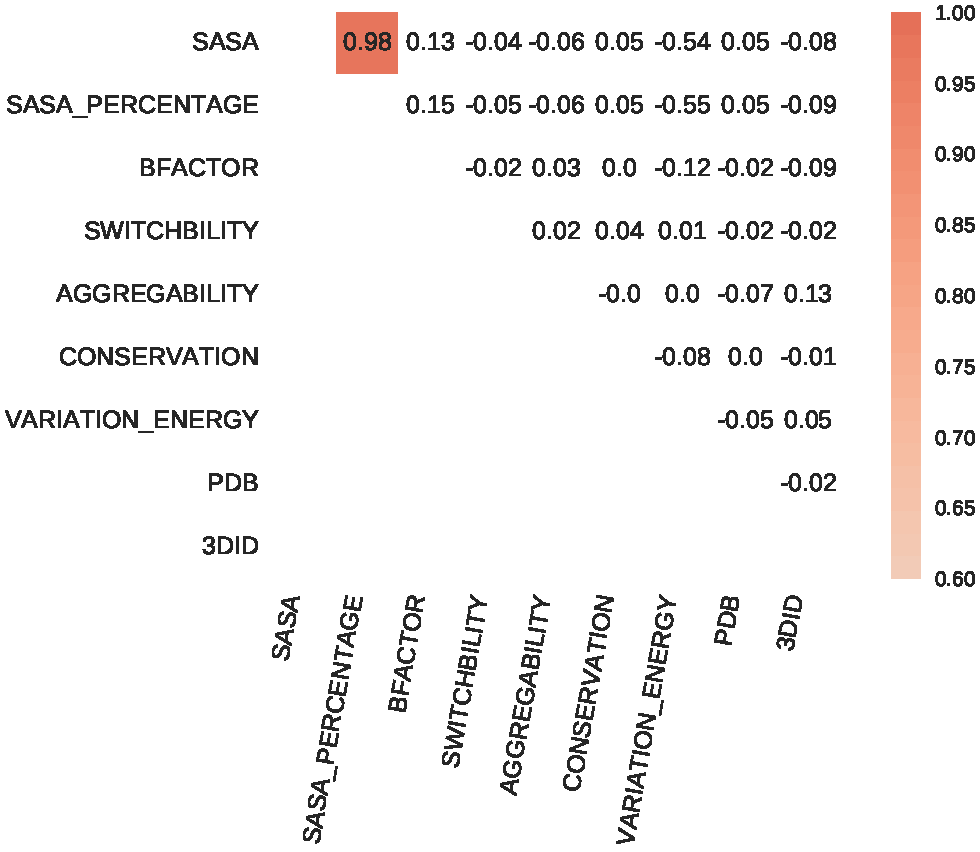
\includegraphics[scale=0.7]{documents/latex/figures/3/varq/varq_corrplot.pdf}
    \caption{Correlación de Spearman para las variables de VarQ Curado.}
    \label{fig:varq_corrplot}
\end{figure}

Finalmente en la tabla \ref{tab:descripcion_varq_cont} podemos ver distintas métricas sobre las variables continuas del dataset, como la media de los valores (mean), el desvío estándar (std), el valor máximo (max) y los cuartiles. 

En esta descripción sumamos el AUC univariado, es decir el área bajo la curva ROC tomando la variable ordenada como estimador de la respuesta.   

Un AUC cercano a 0.5 equivale a una variable de bajo poder predictivo, mientras que un AUC mayor a 0.5 corresponde a un predictor de la variable de respuesta (en este caso una variante patogénica), mientras que un AUC menor a 0.5 corresponde a un anti-predictor, es decir que invertir su respuesta equivale a un predictor de AUC mayor a 0.5. En la columna AUC de la tabla \ref{tab:descripcion_varq_cont} vemos que las variables SASA y SASA \% tienen un poder anti-predictivo relativamente alto (0.34 y 0.33 respectivamente), lo que indica que las variantes que tengan un valor elevado de estas variables tienden a ser benignas, mientras que la variación de energía tiene el mejor poder predictivo univariado entre todas las variables.

\begin{table}[H]
\centering
\begin{tabular}{|l|l|l|l|l|l|l|l|l|}
\hline
Variable & avg  & std   & min    & 25\%  & 50\%  & 75\%  & max & AUC\\ \hline
SASA    & 32.11 & 39.15 & 0.0    & 0.67  & 15.21 & 52.15 & 246.41 & 0.34 \\ \hline
SASA\%  & 0.15  & 0.18  & 0.0    & 0.0   & 0.07  & 0.27  & 0.75 & 0.33  \\ \hline
BFACTOR & 56.45 & 71.76 & 0.0    & 19.77 & 37.34 & 61.14 & 755.61 & 0.46 \\ \hline
SWITCH  & 0.38  & 0.89  & 0.0    & 0.0   & 0.01  & 0.28  & 8.72 &  0.50  \\ \hline
AGG     & 5.02  & 17.61 & 0.0    & 0.0   & 0.0   & 0.16  & 100.0 &  0.51\\ \hline
CONS    & 0.33  & 0.19  & 0.13   & 0.25  & 0.3   & 0.37  & 4.77 & 0.43\\ \hline
ENE     & 2.91  & 4.84  & -12.64 & 0.26  & 1.51  & 3.89 & 57.21 & 0.68\\ \hline 
\end{tabular}
\caption{Descripción de variables continuas del dataset \textit{VarQ Curado}.}
\label{tab:descripcion_varq_cont}
\end{table}

\begin{table}[H]
\centering
\begin{tabular}{|l|l|l|l|}
\hline
Variable & top  & freq. top & BACC \\ \hline
3DID & False & 0.8 & 0.51\\ \hline
PDB  & False  & 0.9 & 0.49\\ \hline
\end{tabular}
\caption{Descripción de variables categóricas del dataset \textit{VarQ Curado}.}
\label{tab:descripcion_varq_cat}
\end{table}

Para el caso de las variables categóricas (PDB y 3DID), analizamos el valor con la frecuencia más alta (top) y el valor de esta frecuencia. Para este tipo de variables quisimos también cuantificar su poder predictivo individual. 

% \newpage

Utilizar AUC en este caso no es posible dado que su cálculo sólo tiene sentido en variables continuas. Por lo tanto, decidimos calcular el \textit{Balanced Accuracy} (BACC) \cite{Brodersen2010} como medida de poder predictivo, considerando el valor de la variable como predictor de la variante.

El \textit{Balanced Accuracy} (BACC) es igual a:
\begin{equation*}
    \frac{1}{2} (\frac{VP}{P} + \frac{VN}{N})
\end{equation*}

Al igual que con el AUC, un valor mucho menor a 0.5 indica poder anti-predictivo, por lo que invertir la respuesta daría lugar a un buen predictor. En la tabla \ref{tab:descripcion_varq_cat} podemos ver que el BACC de las variables 3DID y PDB es de 0.51 y 0.49 respectivamente, lo que indica un bajo valor predictivo. 

% \newpage

\section{Modelo creado a partir del dataset VarQ Curado}

Una vez definido el dataset, podemos emplear técnicas de aprendizaje automático con el objetivo de generar un predictor de variantes patogénicas. Cabe destacar, que en este dataset VarQ Curado hay una sobrerrepresentación de variantes patogénicas, es decir, que presenta un desbalance (mayor número de variantes patogénicas que benignas) que invierte las propociones observadas en el dataset VarQ Completo. De todas formas generaremos un modelo para poder evaluar de forma preliminar la dificultad del problema. 

Para esto recurrimos a diferentes algoritmos de aprendizaje automático: Support Vector Classifier (SVC), Regresión Logística y Random Forest. La construcción del pipeline para cada uno de estos algoritmos constó de tres fases: 

\begin{itemize}
    \item \textbf{Creación del set de entrenamiento y de evaluación}: División (\textit{split}) estratificado (es decir, manteniendo las proporciones originales de la variable objetivoE) del dataset, 66\% para entrenamiento y 33\% para evaluación. 
    \item \textbf{Imputación de las variables}: Se reemplazaron los valores nulos de cada variable por su mediana en caso de las continuas y por el valor más frecuente en el caso de las variables categóricas.
    \item \textbf{Estandarización}: Para el caso de los algoritmos paramétricos (Regresión Logística y SVM) se aplicó una estandarización robusta a outliers. Esta estandarización consiste en restar la mediana del valor y escalar los datos de acuerdo a la distancia intercuartil, como se observa en la ecuación \ref{eq:robust_scaler}.
    
    \begin{equation}
        RobustScaling(x_i) = \frac{x_i - Q_2(\textbf{x})}{Q_3(\textbf{x}) - Q_1(\textbf{x})} 
        \label{eq:robust_scaler}
    \end{equation}
    
    donde $x_i$ corresponde al valor de la variable,  $Q_1$, $Q_2$ y $Q_3$ corresponde al primer, segundo y tercer cuartil de la variable $\textbf{x}$ respectivamente.
    
    
\end{itemize}

Luego del preprocesamiento, para cada uno de los algoritmos se realizó una búsqueda de hiperparámetros óptimos, a partir de estos datos, con la función \texttt{GridSearchCV} de la biblioteca \texttt{Scikit-learn} \cite{scikit-learn}. El objetivo de esta función es evaluar todas las combinaciones de hiperparámetros definidos en un diccionario y retornar el estimador que dio mejores resultados (de acuerdo a una métrica escogida, en este caso el área bajo la curva ROC). Esta métrica a su vez es evaluada a través de validación cruzada (\textit{3-fold Cross Validation}). En el apéndice se encuentran los diccionarios de hiperparámetros usados en cada uno de los modelos.

\section{Resultados}

Random Forest fue el mejor modelo con un AUC de 0.74. Los parámetros óptimos de este modelo fueron una profundidad de árbol de 7, 100 estimadores y una cantidad máxima de variables por árbol de 4. Denominaremos este modelo como Modelo VarQ Curado.

La Regresión Logística y SVC obtuvieron 0.71 y 0.70 de AUC respectivamente. Estos modelos se caracterizaron ademas por tener una tendencia a clasificar a las variantes como patogénicas, lo que se puede observar en su alto recall y menor precisión con respecto a Random Forest. En particular, SVC clasificó a todas las variantes del dataset de evaluación como patogénicas. También el tiempo de entrenamiento fue mucho mayor que el del resto de los algoritmos. En la tabla \ref{tab:metricsmodel} presentamos la Precisión y el Recall (con respecto a las variantes patogénicas) y el tiempo de entrenamiento del modelo y de predicción de todas las variantes del dataset de evaluación.

\begin{table}[H]
\centering
\begin{tabular}{|l|l|l|l|l|l|l|}
\hline
Modelo & Precisión & Recall & AUC & F1-score & $t_{fit}$ & $t_{pred}$ \\ \hline
SVC    & 0.72 & \textbf{1.00} & 0.70 & 0.84 & 2 m 39 s & 0.77s \\ \hline
LR     & 0.75 & 0.94 & 0.71 & 0.84 & \textbf{1.17 s} & \textbf{0.01 s} \\ \hline
RF     & \textbf{0.77} & 0.93 & \textbf{0.74} & 0.84 & 9.82 s & 0.11 s \\ \hline
\end{tabular}
\caption{Comparación de métricas de modelos usando el dataset VarQ Curado. Las variables $t_{fit}$ y $t_{pred}$ corresponden al tiempo de entrenamiento y de predicción de todas las variantes.}
\label{tab:metricsmodel}
\end{table}

La tabla \ref{tab:metrics_varq} muestra algunas métricas de interés obtenidas del modelo Random Forest para entender mejor los resultados del modelo basados en el predictor generado.

\begin{table}[H]
\centering
\begin{tabular}{|l|l|l|l|}
\hline
              & Precisión & Recall & F1-score \\ \hline
Benignas      & 0.57      & 0.26   & 0.36     \\ \hline
Patogénicas   & 0.77      & 0.93   & 0.84     \\ \hline
Promedio      & 0.71      & 0.74   & 0.71     \\ \hline
\end{tabular}
\caption{Reporte de métricas del modelo Random Forest usando el dataset VarQ Curado.}
\label{tab:metrics_varq}
\end{table}

La precisión del modelo indica un número marcadamente bajo (0.57) en la clase benigna, lo que significa que casi una de cada dos variantes detectadas como benignas es en efecto patogénica. El Recall con respecto a las variantes benignas es de 0.26, es decir que el modelo sólo reconoce alrededor de un cuarto de las variantes benignas como tales. Por lo tanto podemos afirmar que este modelo tiene una tendencia a clasificar las variantes como patogénicas, generando una gran cantidad de falsos positivos (o Error de tipo I). Es importante remarcar que estas métricas están generadas a partir de una función de decisión o \textit{threshold} fijado por la versión del algoritmo usado (en el caso de la biblioteca \texttt{scikit-learn}, este \textit{threshold} está ubicado en 0.5 de la probabilidad asignada).  La curva ROC, o \textit{Receiver Operating Characteristic} y su AUC asociada, nos permite independizarnos de un \textit{threshold} fijo para evaluar las características del predictor (figura \ref{fig:auc_varq}).

En la figura \ref{fig:importance_varq} podemos observar la importancia de los features reportado por el algoritmo Random Forest, que ubica en primer lugar con una gran diferencia a la variable que hace referencia a la Variación de Energía (ENE), seguido por el BFACTOR y el porcentaje de SASA (SASA \%). Este dato concuerda parcialmente con sus valores de AUC univariado (tabla \ref{tab:descripcion_varq_cont}). Si bien ENE y SASA \% poseen un valor relativamente alto de poder de clasificación univariada, no sucedía lo mismo con BFACTOR. En el modelo multivariado esta situación se invierte, con BFACTOR en el segundo lugar de importancia.

\newpage

\begin{figure}[H]
\centering
\begin{subfigure}{0.7\textwidth}
    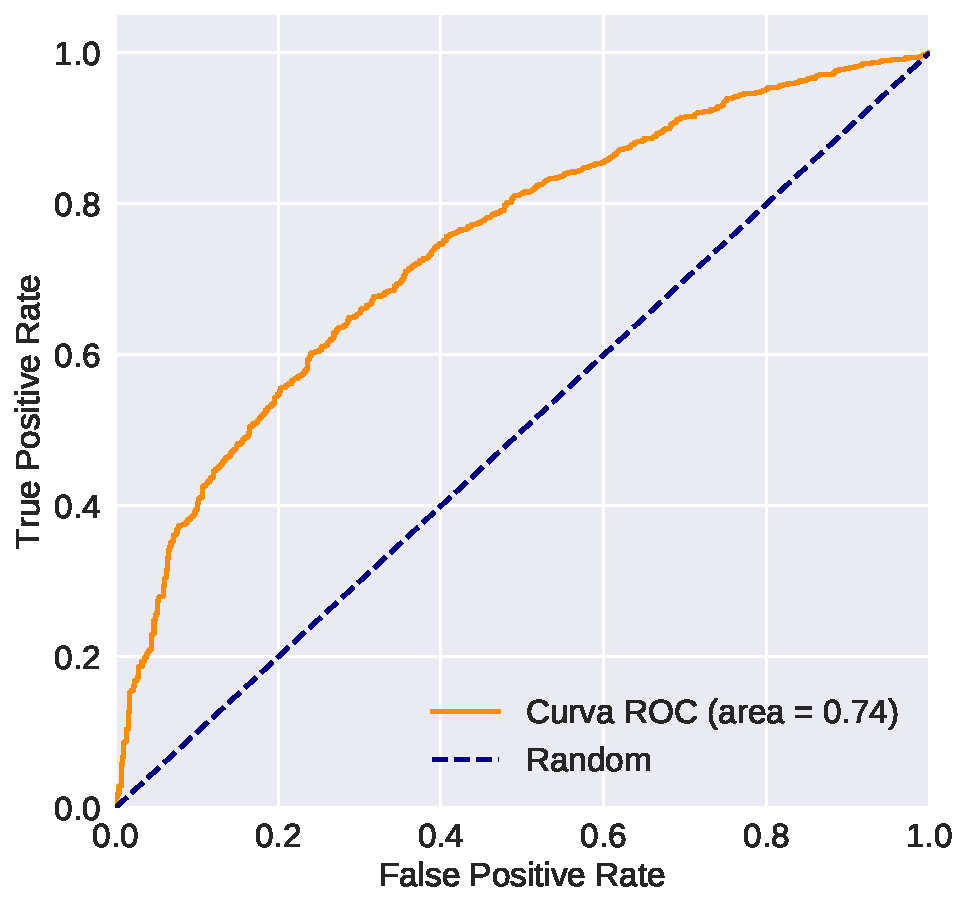
\includegraphics[width=\textwidth]{documents/latex/figures/3/varq/auc_varq.pdf}
    \caption{Curva ROC del modelo. La línea punteada corresponde a la curva ROC de un estimador aleatorio, o \textit{Random}, cuyo AUC es igual a 0.5.}
    \label{fig:auc_varq}
\end{subfigure}
\begin{subfigure}{0.7\textwidth}
    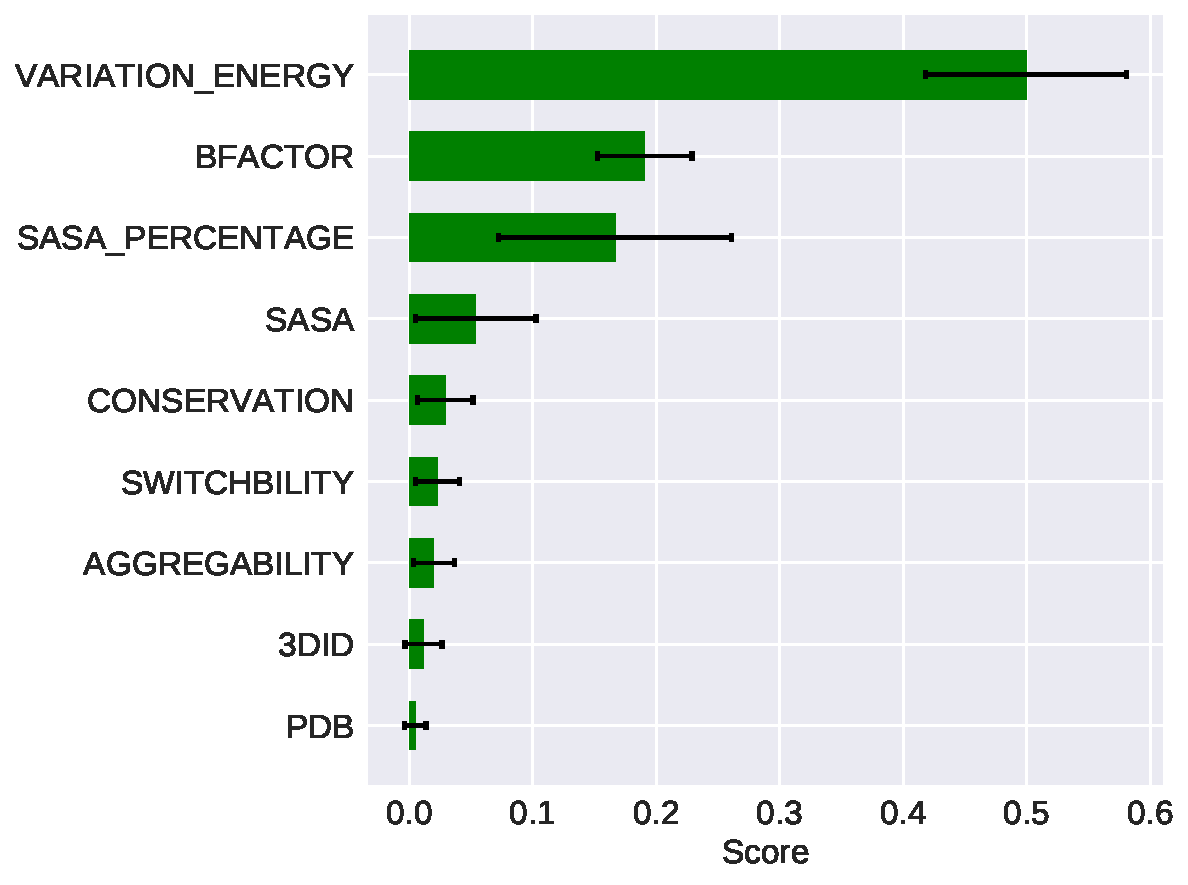
\includegraphics[width=\textwidth]{documents/latex/figures/3/varq/importances_varq.pdf}
    \caption{Los atributos del dataset VarQ Curado en orden de importancia. La barra de error corresponde al desvío estándar del \textit{Feature Importance} de cada uno de los árboles del modelo.}
    \label{fig:importance_varq}
\end{subfigure}

\caption{Curva AUC y atributos más importantes del Modelo VarQ Curado.}

\end{figure}